\documentclass[../main]{subfiles}
\usepackage{lastpage,xr,refcount,etoolbox}
% \externaldocument{references}
\begin{document}


\chapter{The Setup of the Project}

{
\hypersetup{linkcolor=black}
\minitoc
}

\section{YOLO, the model}
YOLO, which stands for "You Only Look Once," is a popular real-time object detection system. It is widely used in computer vision tasks because of its high speed and accuracy in detecting objects within images and videos. Here's a detailed overview of YOLO:

\begin{itemize}
    \item[\textbullet] \textbf{Single Neural Network Approach}: Unlike traditional object detection systems that use a pipeline of separate models for region proposal and classification, YOLO uses a single convolutional neural network (CNN) to predict multiple bounding boxes and class probabilities directly from the full images in one evaluation.
    \item[\textbullet] \textbf{Real-time Detection}: YOLO is designed to process images extremely quickly, making it suitable for real-time applications. For instance, YOLO can achieve frame rates of up to 45 frames per second (fps) on a modest GPU.
    
\end{itemize}
YOLOv8 represents the latest iteration in the YOLO (You Only Look Once) series of object detection models. As a continuation of the YOLO family, YOLOv8 builds upon the advancements made by its predecessors, enhancing both speed and accuracy. Here’s a detailed look at what makes YOLOv8 stand out, particularly the yolov8x.pt model.
\subsection{Why yolov8n.pt?}
The model yolov8n.pt is one of the variants in the YOLOv8 family, and the name conveys specific information about its characteristics:
\begin{itemize}
\item[\textbullet] \textbf{yolov8}: This prefix denotes that the model is part of the YOLO version 8 series. It indicates the architecture and the improvements over earlier YOLO versions.
\item[\textbullet] \textbf{n}: This letter stands for “nano” and signifies that the model is designed with a smaller capacity compared to its larger counterparts like yolov8s (small) or yolov8m (medium). In the context of YOLOv8, the n variant offers fewer parameters, which can lead to faster inference and lower resource consumption while maintaining reasonable detection accuracy and robustness.
\item[\textbullet] \textbf{.pt}: This suffix indicates that the model is saved in PyTorch format. PyTorch is a popular deep learning framework that provides flexibility and ease of use for training and deploying models.
\end{itemize}
Even though yolov8n is a "nano" model, it is designed to be highly efficient and lightweight. In fact, yolov8n.pt is an excellent choice, especially when computing resources are limited because it is a well-balanced model that provides strong performance for object detection tasks without being overly demanding on computing resources. Its advanced architecture and optimizations make it an excellent choice for projects where efficiency and effectiveness are key, especially when working with constrained computational environments. In the case of training for hand detection in a Rock-Paper-Scissors application, yolov8n.pt offers a pragmatic solution by delivering the necessary accuracy and speed to recognize hand gestures while being well-suited for deployment on devices with limited hardware capabilities.

\begin{figure}[H]
   \centering
   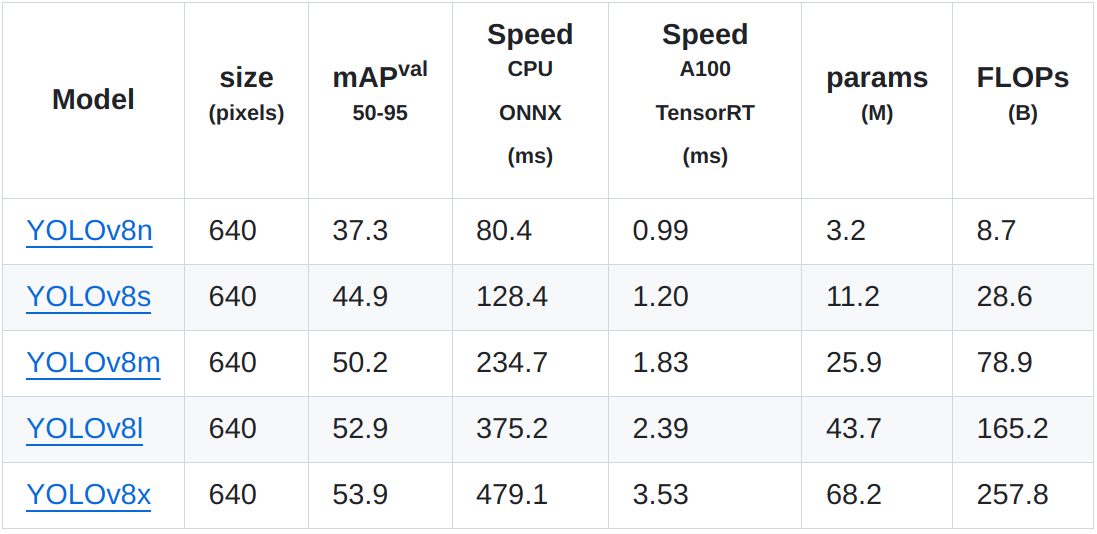
\includegraphics[width=0.8\textwidth]{./figures/imagen1}
   \caption{Rock paper scissors game}
 \label{fig:red}
\end{figure}

Moreover, the choice of yolov8n.pt for training a hand detection model in a Rock-Paper-Scissors application underscores a strategic balance between model efficiency and performance. The YOLOv8n variant’s reduced parameter count and optimized architecture are particularly advantageous for real-time applications, where processing speed and responsiveness are crucial. Its lightweight design ensures that the model can be deployed effectively on edge devices with constrained resources, such as mobile phones or embedded systems, without compromising on detection accuracy. By leveraging the PyTorch framework’s capabilities, yolov8n.pt facilitates streamlined development and deployment workflows, enabling rapid iterations and adjustments as needed. This makes it an ideal candidate for practical implementations where maintaining a high level of performance while minimizing computational overhead is essential.
\section{How to prepare the dataset}
Regardless of whether you are using YOLO 5, 7, or 8, the format of the dataset remains the same. In other words, if you have already prepared your dataset for training an older YOLO model, you can reuse it to train a newer version. As we already said, we are going to train the YOLO model "yolov8n.pt" because it is lightweight with fewer parameters, allowing the training process to be faster while still maintaining good performance.

If you don't already have a dataset prepared to train your model, you can use the services of Roboflow to create one from scratch. However, be aware that if you are working alone, the process of obtaining your custom dataset can be extremely tedious.

\subsection{Structure of the Dataset}
Before we dive into how to obtain your own custom dataset, let's first explain the file structure you need and the configuration files required. Firstly, we need to organize our dataset into a specific directory structure. A common structure could look like this:

\begin{lstlisting}
/name_dataset
    /all_images
        image1.jpg
        image2.jpg
        ...
        image.png
           
    /all_labels
        image1.txt
        image2.txt
        ...
        image.txt
\end{lstlisting}
In the all\_images folder, you'll find each image you plan to use in your dataset. In the all\_labels folder, you'll find a .txt file for each corresponding image. Let's examine the contents of one of these .txt files:
\begin{lstlisting}
6 0.72475961538 0.3209134615 0.3846153846 0.59134615384
\end{lstlisting}
At first glance, it might not be clear what these numbers represent. To clarify, here's the general format for a .txt file:
\begin{lstlisting}
<class_id> <x_center> <y_center> <width> <height>
\end{lstlisting}
Here's what each value represents:
\begin{itemize}
    \item[\textbullet] \textbf{$<$class\_id$>$}: Integer representing the class of the object (starting from 0).
    \item[\textbullet] \textbf{$<$x\_center$>$}: Normalized x-coordinate of the center of the bounding box (value between 0 and 1).
    \item[\textbullet] \textbf{$<$y\_center$>$}: Normalized y-coordinate of the center of the bounding box (value between 0 and 1).
    \item[\textbullet] \textbf{$<$width$>$}: Normalized width of the bounding box (value between 0 and 1).
    \item[\textbullet] \textbf{$<$height$>$}: Normalized height of the bounding box (value between 0 and 1).
\end{itemize}

\subsection{Obtain your dataset with Roboflow}
Roboflow \hyperlink{target:zona}{\textcolor{blue}{[2]}} is a platform designed to help users build, manage, and deploy computer vision models. It provides tools and services that simplify the process of preparing data, training models, and integrating those models into applications. Once you have an account, you can create a new project and specify the classes you want the model to identify: 
\begin{figure}[H]
   \centering
   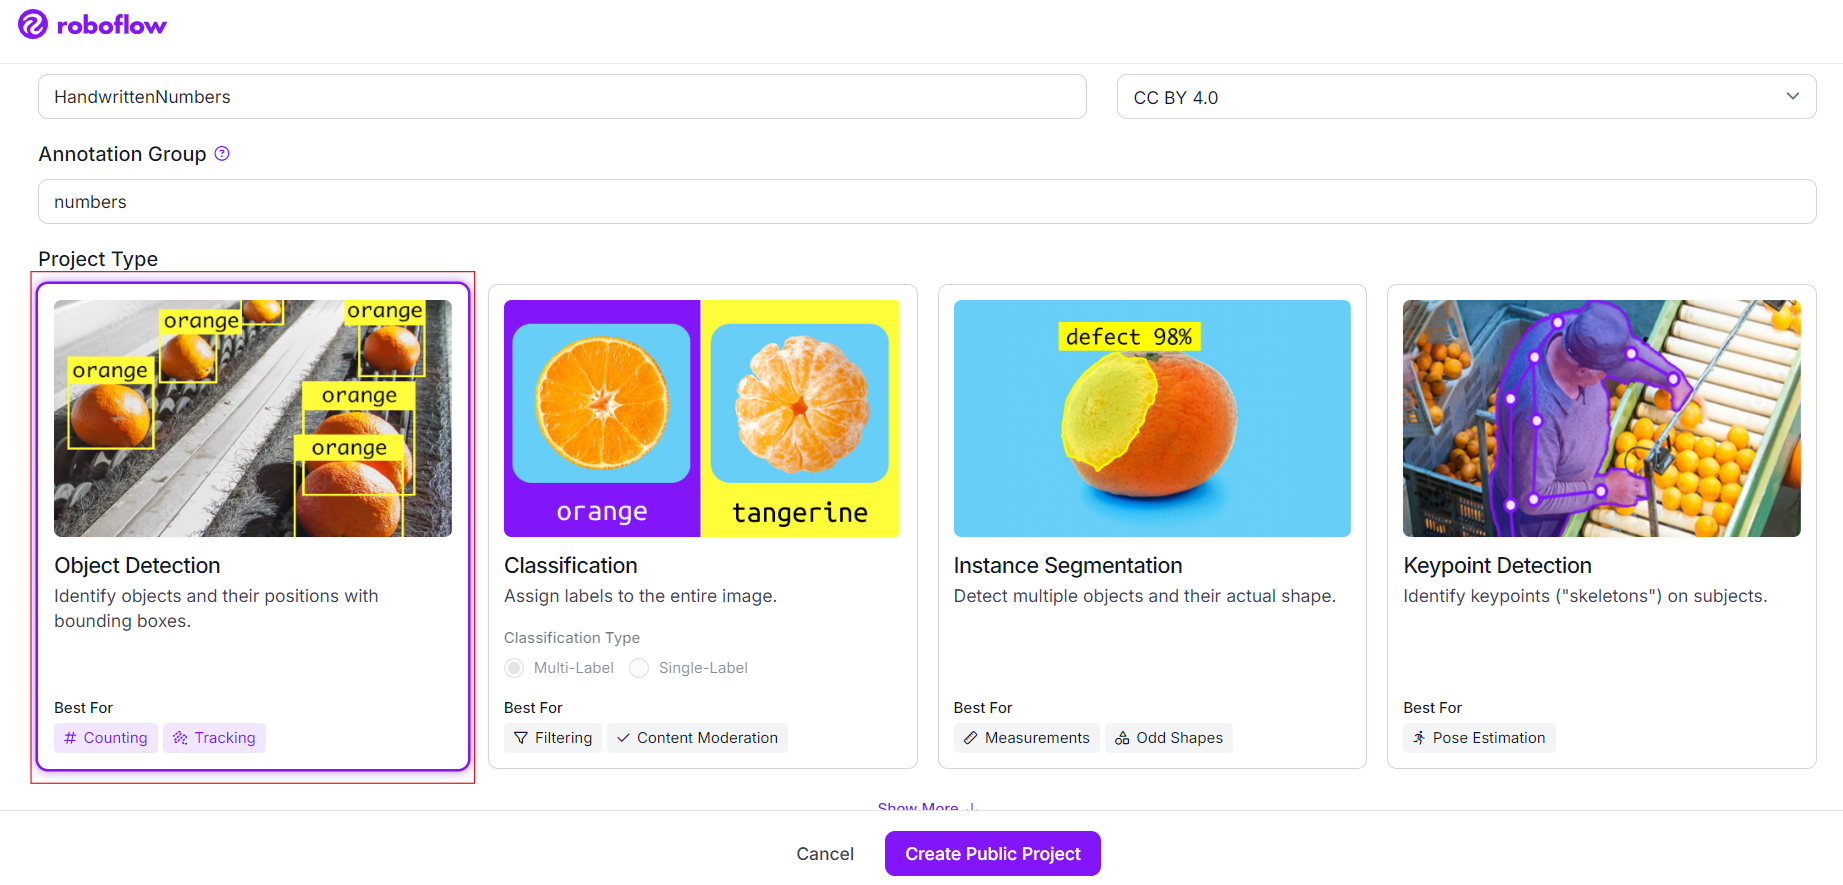
\includegraphics[width=0.7\textwidth]{./figures/roboflowProject}
   \caption{Create a project in Roboflow}
 \label{fig:red}
\end{figure}
Once you have created the project, you can upload or drag and drop all the images you want to use for your dataset. Depending on the number and quality of the images, this may take a moment. After uploading, you'll have the option to manually label the images, collaborate with others to label them, or use a custom model to assist with labeling. Since we do not have a custom model, the alternative will be to manually label the images.
\begin{figure}[H]
    \centering
    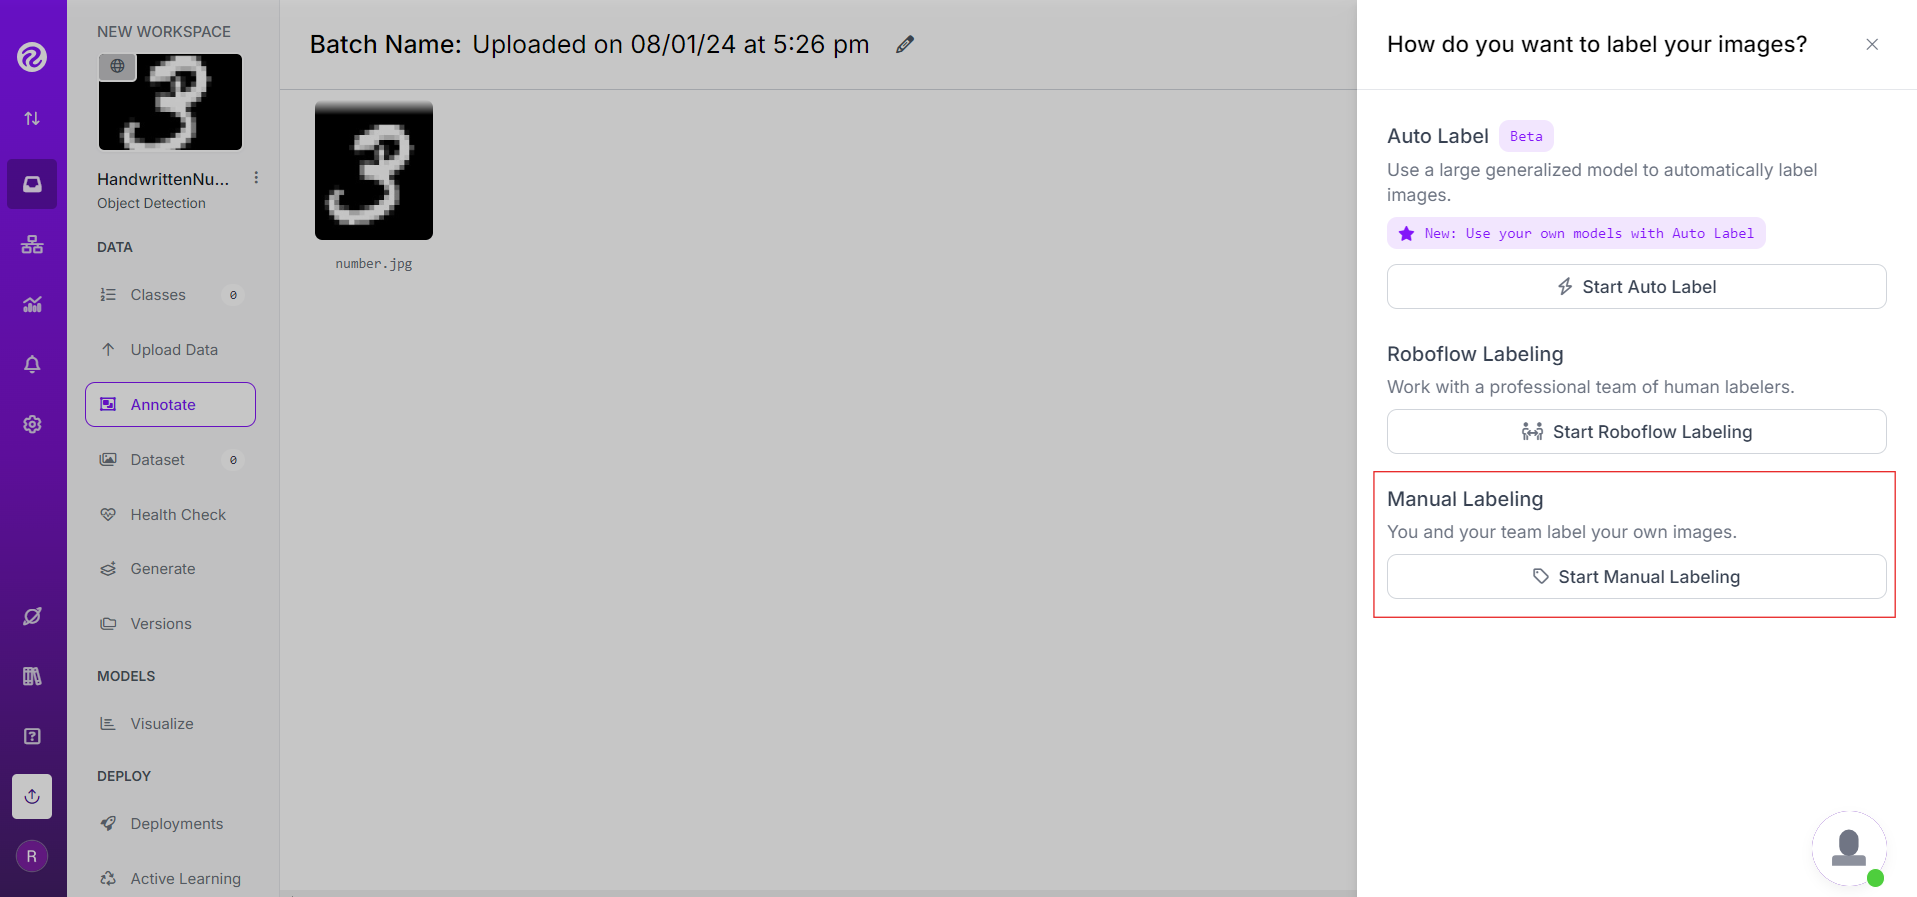
\includegraphics[width=1\textwidth]{./figures/label}
    \caption{How to label the images?}
    \label{fig:red}
\end{figure}
Once you have done so, the next step is straightforward: to manually label each image and determine the class it belongs to. Here’s an example of how this is done: 
\begin{figure}[H]
        \centering
        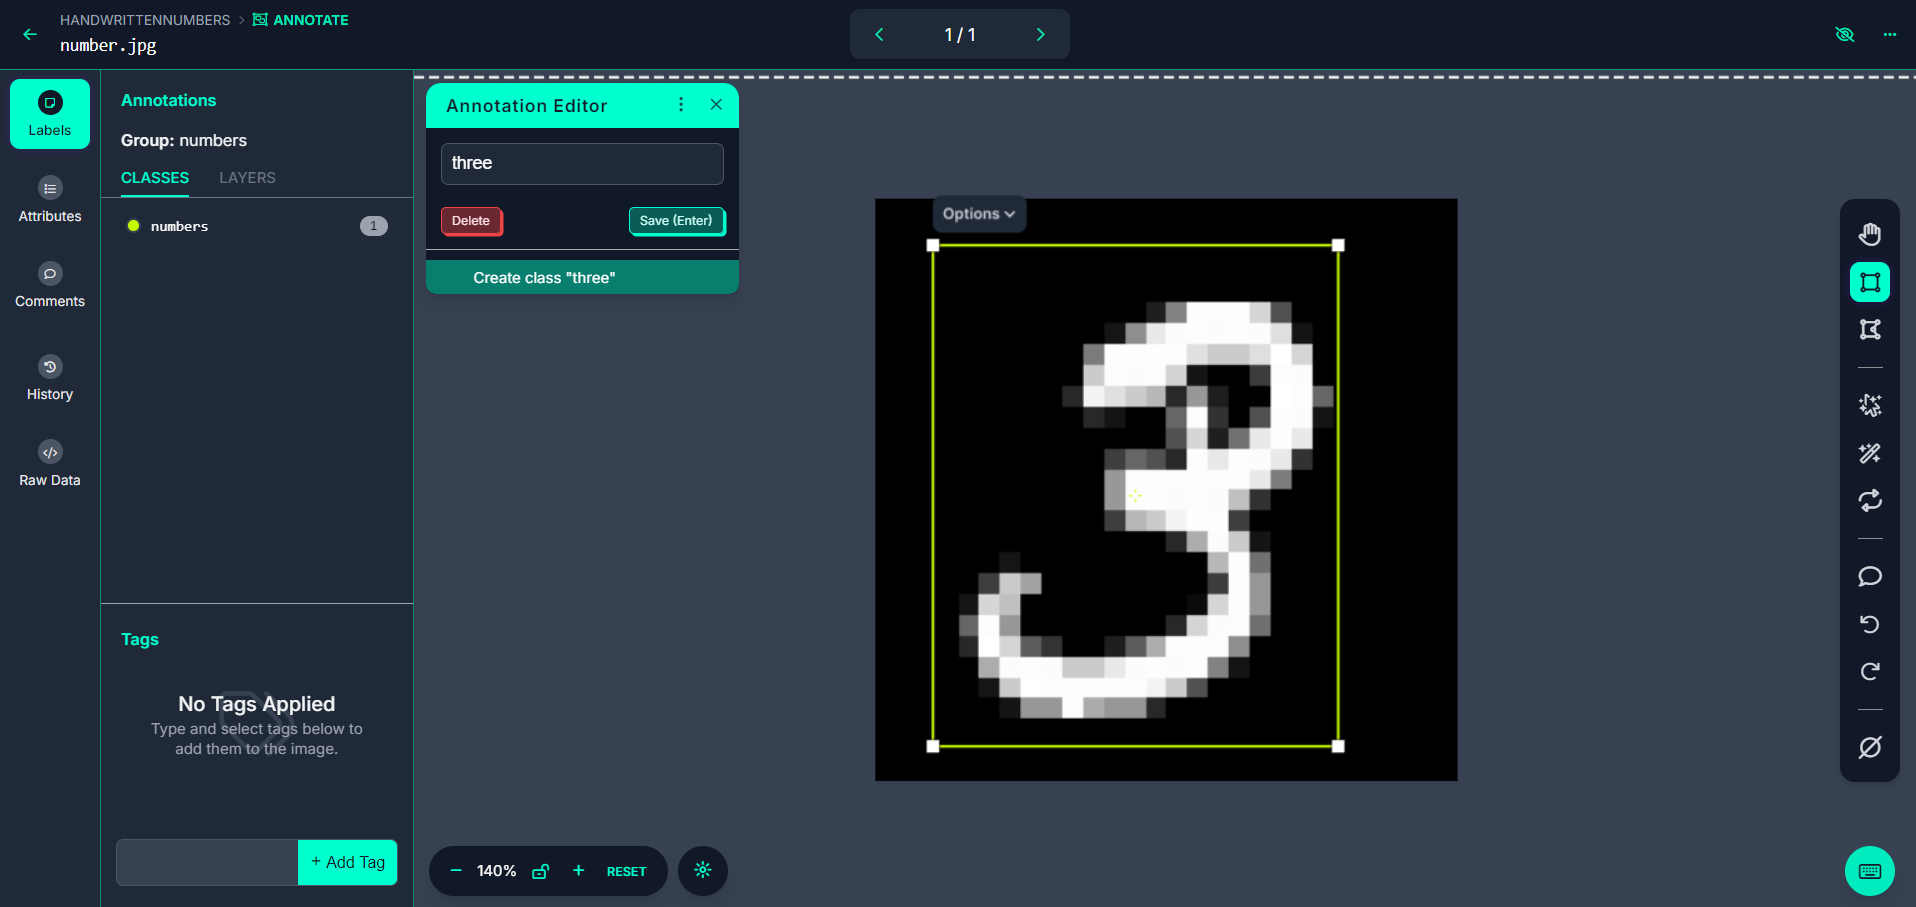
\includegraphics[width=1\textwidth]{./figures/three}
        \caption{Label of a 3}
        \label{fig:red}
\end{figure}
Once we have labeled all the images correctly (for a large dataset, we can manually annotate the initial images, train a model, and then use that model to annotate the rest. After several iterations, we will end up with a robust model), the next step is to choose the percentages for splitting the dataset into training, validation, and testing sets.
\begin{figure}[H]
      \centering
      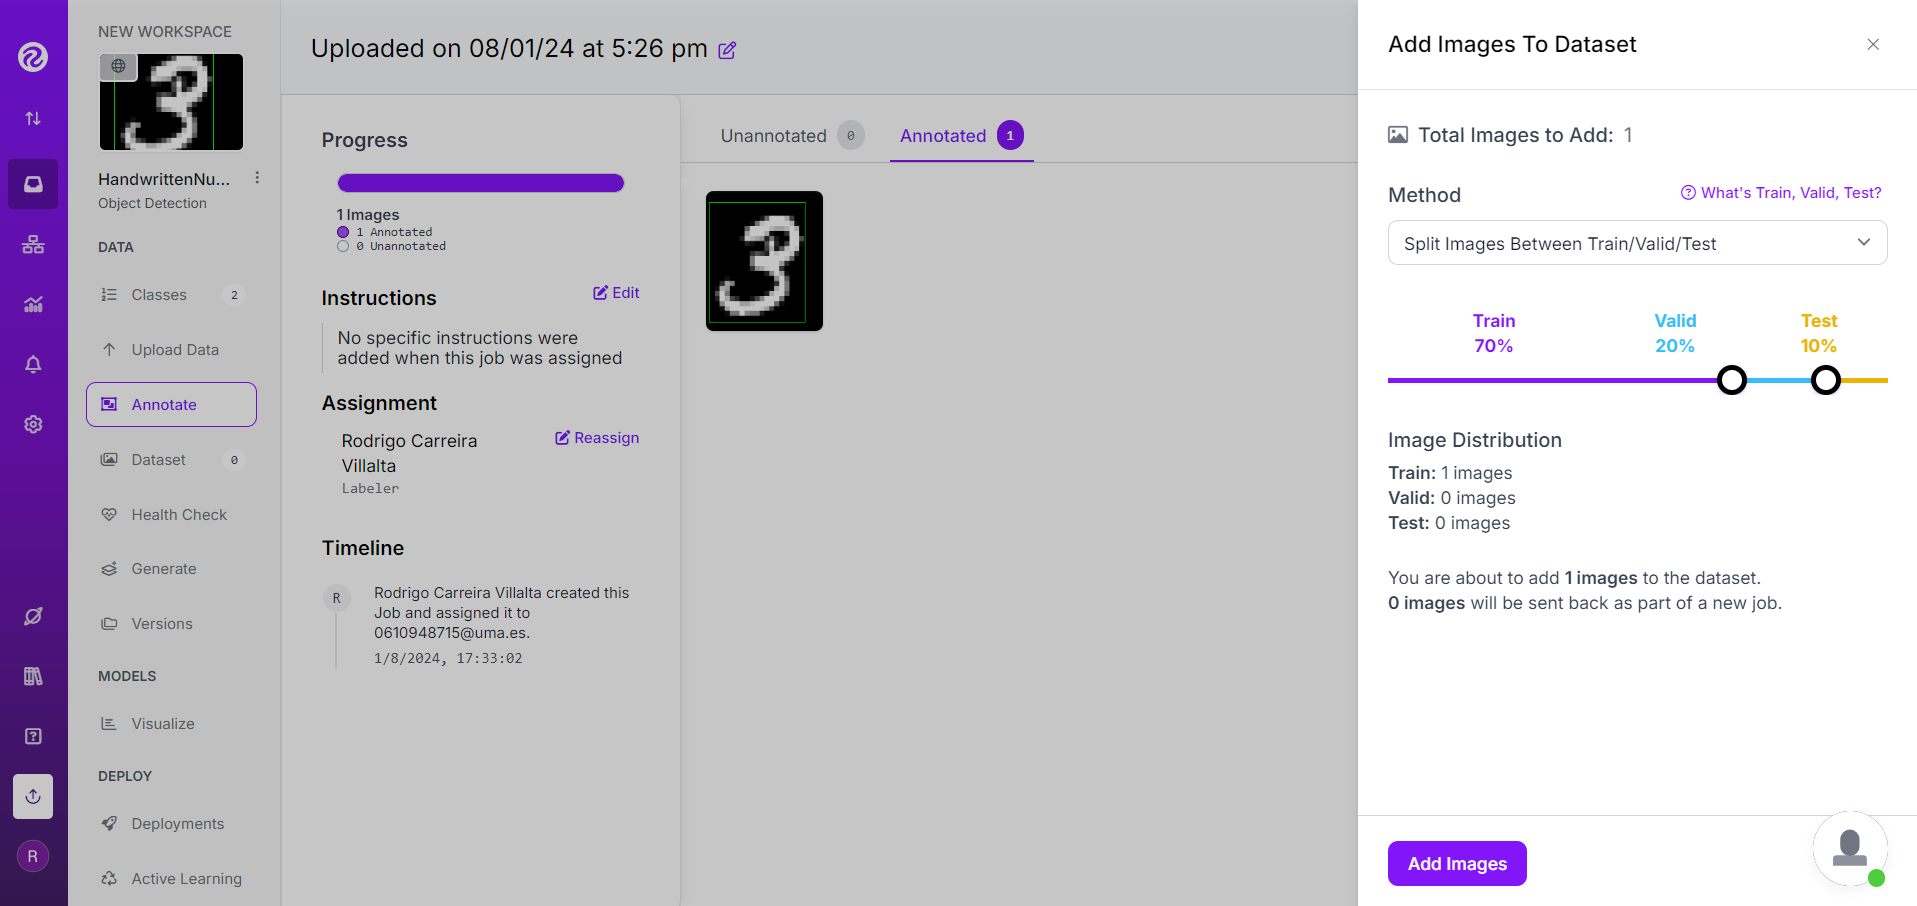
\includegraphics[width=1\textwidth]{./figures/train}
      \caption{Percentages for train, validate and test}
      \label{fig:red}
\end{figure}
Once everything is done, it's time to create the dataset in YOLO format. Roboflow will ask if you want to add any preprocessing, augmentation, or other modifications. This decision is up to you. After configuring these options, click on "Create" to generate your dataset in the YOLO format:
\newpage
\begin{figure}[H]
     \centering
     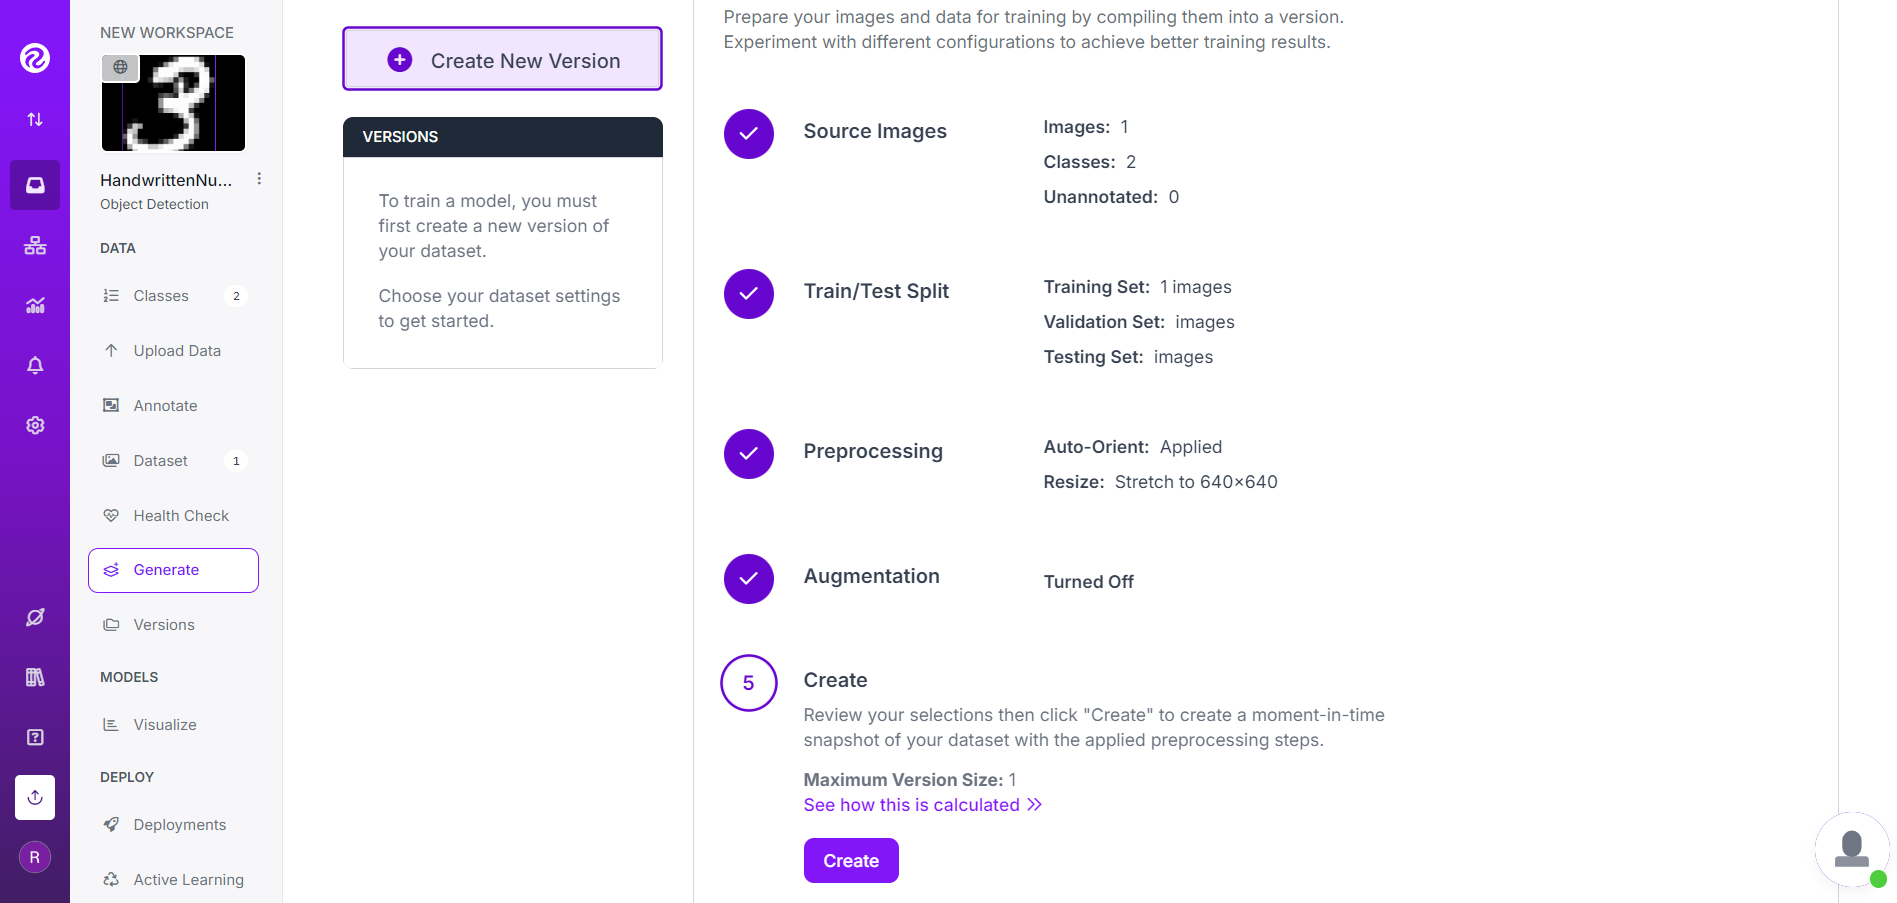
\includegraphics[width=1\textwidth]{./figures/create}
     \caption{Obtaining Our YOLO-Formatted Dataset}
     \label{fig:red}
\end{figure}
\subsection{Configuration files}
The real importance of getting a .txt file for every image in our dataset is to be able to finally obtain a bag of files indicating the geometrical position of the detections in each of the images. At the end of this whole process, the data structure is composed of two folders: "images" and "labels". In our case, they both are included in a "dataset.zip" file, which is unzipped by our Python script.

Once the "dataset.zip" file is unzipped, we obtain two folders, but what should we do with them? The answer is in the Ultralytics Documentation. YOLO models are designed to be trained with .yaml files. YAML is a human-readable data serialization language. It is commonly used for configuration files and in applications where data are being stored or transmitted. In our case, our configuration.yaml file will specify where the training split, validation split, and testing split are located. That’s all! Our Python script will take care of both making these splits into the three different folders needed, as well as creating the .yaml file. Its format will be as follows:
\begin{lstlisting}
path: "your_computer_path\dataset_split"
train: train
val: val
test: test

nc: 3
names: ['paper', 'rock', 'scissors']
\end{lstlisting}

Finally, the whole structure of the folders that our `yolov8n.pt` model will use to train itself will be something like this:

\begin{lstlisting}
/dataset
    /train
        /images
            image1.jpg
            image2.jpg
            ...
        /labels
            image1.txt
            image2.txt
            ...
    /val
        /images
            image11.jpg
            image22.jpg
            ...
        /labels
            image11.txt
            image22.txt
            ...
    /test
        /images
            image111.jpg
            image222.jpg
            ...
        /labels
            image111.txt
            image222.txt
            ...
\end{lstlisting}

Some of the images found in the "images" folder will look like the following, and as you can see, not all the images will be easy for our YOLO model. For example, Figure 1.7 shows a restaurant image where YOLOv8n has to detect nothing:

\begin{figure}[H]
    \centering
    \begin{minipage}{0.48\textwidth}
        \centering
        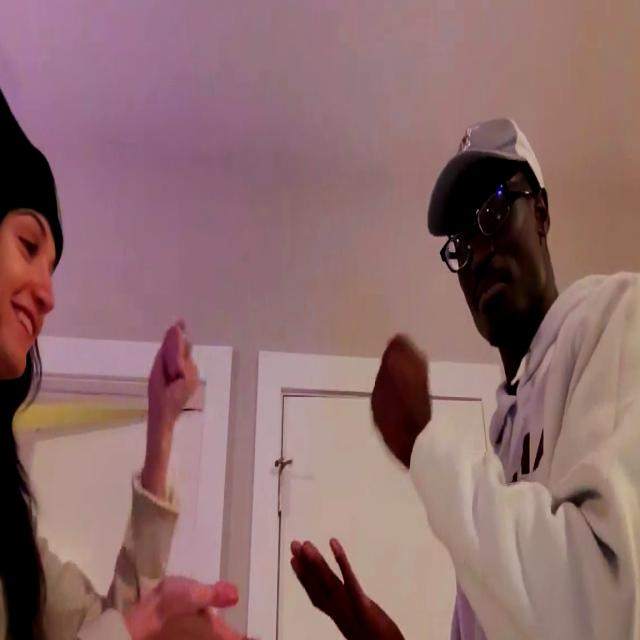
\includegraphics[width=\linewidth]{./figures/0058_png.rf.8ce89ad8eaffb9cda78bfbdbafa0bc4e}
        \caption{Dataset image: Example 1}
        \label{fig:example1}
    \end{minipage}\hfill
    %\hspace{0.01\textwidth} % Ajusta este valor según sea necesario para la separación
    \begin{minipage}{0.48\textwidth}
        \centering
        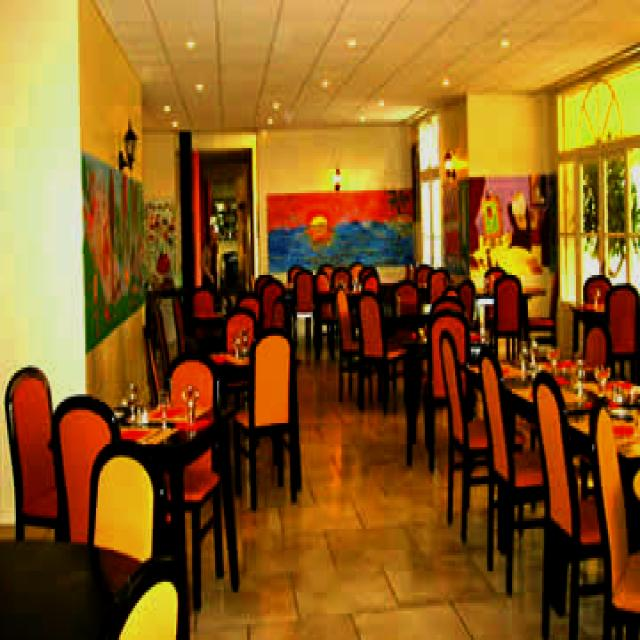
\includegraphics[width=\linewidth]{./figures/40_salle_restaurant_jpg.rf.78cf734a80c15db11168024464278a57}
        \caption{Dataset image: Example 2}
        \label{fig:example2}
    \end{minipage}
\end{figure}


\newpage

\subsection{The dataset of this project}
As most readers might have already deduced, the most tedious and time-consuming process is obtaining the dataset for training the model. Fortunately, for this project, we have a great resource available: a public dataset from Roboflow for rock-paper-scissors image recognition. This dataset provides a large collection of images already labeled and ready for use, saving us the effort of manual labeling. Using this dataset will allow us to focus on the learning aspects of the project and developing the image recognition model.

This significantly shortens the time we would have spent manually labeling each image using tools like Roboflow. Instead, we are left with the tasks of setting up the file structure, preparing the configuration files, and writing the Python script needed to prepare the dataset for model training.

\subsubsection{Script to prepare the Dataset}
Now it’s time to break down the code used in the project to prepare the public Roboflow dataset for rock-paper-scissors image recognition and train our YOLO model. First, we start with the necessary imports and define the paths where our dataset is located and where it will be organized:

\begin{lstlisting}
import cv2
import os
import sys
from ultralytics import YOLO
import shutil
import random
from zipfile import ZipFile

cd = os.getcwd()                    # it's gonna be /src
base_path = 'dataset_split'
\end{lstlisting}
Secondly, we have an auxiliary function that moves files to their respective directories based on the dataset split.
\begin{lstlisting}
def move_files(data, split, images_path, labels_path):
    for img_file, lbl_file in data:
        shutil.move(os.path.join(images_path, img_file), os.path.join(base_path, split, 'images', img_file))
        
        shutil.move(os.path.join(labels_path, lbl_file), os.path.join(base_path, split, 'labels', lbl_file))
\end{lstlisting}
Lastly, we have a function that sets up the directory structure, splits the dataset into training, validation, and test sets, and moves the files accordingly using the auxiliary function described earlier:

\newpage
\begin{lstlisting}
def prepare_structure():
    # Define paths
    zip_file_path = 'dataset.zip'
    base_extract_path = 'dataset'
    url = 'drive_url_with_dataset'
    ...
    with open(os.path.join(base_path, 'config.yaml'), 'w') as file:
        file.write(config_content)

    print("Data distribution and yaml creation completed successfully ...")
\end{lstlisting}
Lastly, we implemented two auxiliary functions to remove the entire folder structure if the user decides to do so:
\begin{lstlisting}
def remove_empty_dirs(path):
    for dirpath, dirnames, filenames in os.walk(path, topdown=False):
        if not dirnames and not filenames:
            os.rmdir(dirpath)

    # Attempt to remove the base directory
    try:
        os.rmdir(path)
    except OSError as e:
        print()

def removeAll():
    if os.path.exists(f"{cd}/dataset_split"):
        shutil.rmtree(f'{cd}/dataset_split', ignore_errors=True)
        print("Data distribution deleted successfully ...")
    ...
    else:
        print(f"The directory {cd}/dataset does not exist.")
\end{lstlisting}


\end{document}


%\hyperlink{target:zona}{\textcolor{blue}{[2]}} 